\begin{frame}
 \frametitle{Line from Two Points}
Given: distinct points $P_0$ and $P_1$, with position vectors $\textbf{r}_0$ and $\textbf{r}_1$. \\

$L$: line through $P_0$ and $P_1$.

\bigskip

\begin{columns}
  \column{6cm}

  \uncover<2->{Direction of $L$: $\textbf{u} = \textbf{r}_1 - \textbf{r}_0$.\\}
  \uncover<5->{$\textbf{u} = \langle x_1-x_0,y_1-y_0,z_1-z_0\rangle$}

  \uncover<3->{\medskip \textcolor[rgb]{0.98,0.00,0.00}{Parametric vectorial equation} of $L$:\\
  $\textbf{r} = \textbf{r}_0 + t(\textbf{r}_1-\textbf{r}_0)$\\}

  \uncover<4->{\medskip Equivalent equation:\\
  $\textbf{r} = (1-t)\textbf{r}_0 + t\textbf{r}_1$}
  \column{6cm}
    \only<2-4>{\begin{figure}
        \psfrag{O}{$O$}
        \psfrag{L}{$L$}
        \psfrag{P}{$P$}
        \psfrag{P0}{$P_0$}
        \psfrag{P1}{$P_1$}
        \psfrag{r}{$\textbf{r}$}
        \psfrag{u}{$\textbf{u}$}
        \psfrag{r0}{$\textbf{r}_0$}
        \psfrag{r1}{$\textbf{r}_1$}
        \includegraphics[height=1.5in]{../../modules/vectors/pictures/ok-line_point_point_vector.eps}
    \end{figure}}
    \only<5->{\begin{figure}
        \psfrag{O}{$O$}
        \psfrag{x}{$x$}
        \psfrag{y}{$y$}
        \psfrag{z}{$z$}
        \psfrag{L}{$L$}
        \psfrag{P}{$P(x,y,z)$}
        \psfrag{P0}{$P_0(x_0,y_0,z_0)$}
        \psfrag{P1}{$P_1(x_1,y_1,z_1)$}
        \psfrag{r}{$\textbf{r}$}
        \psfrag{u}{$\textbf{u}$}
        \psfrag{r0}{$\textbf{r}_0$}
        \psfrag{r1}{$\textbf{r}_1$}
        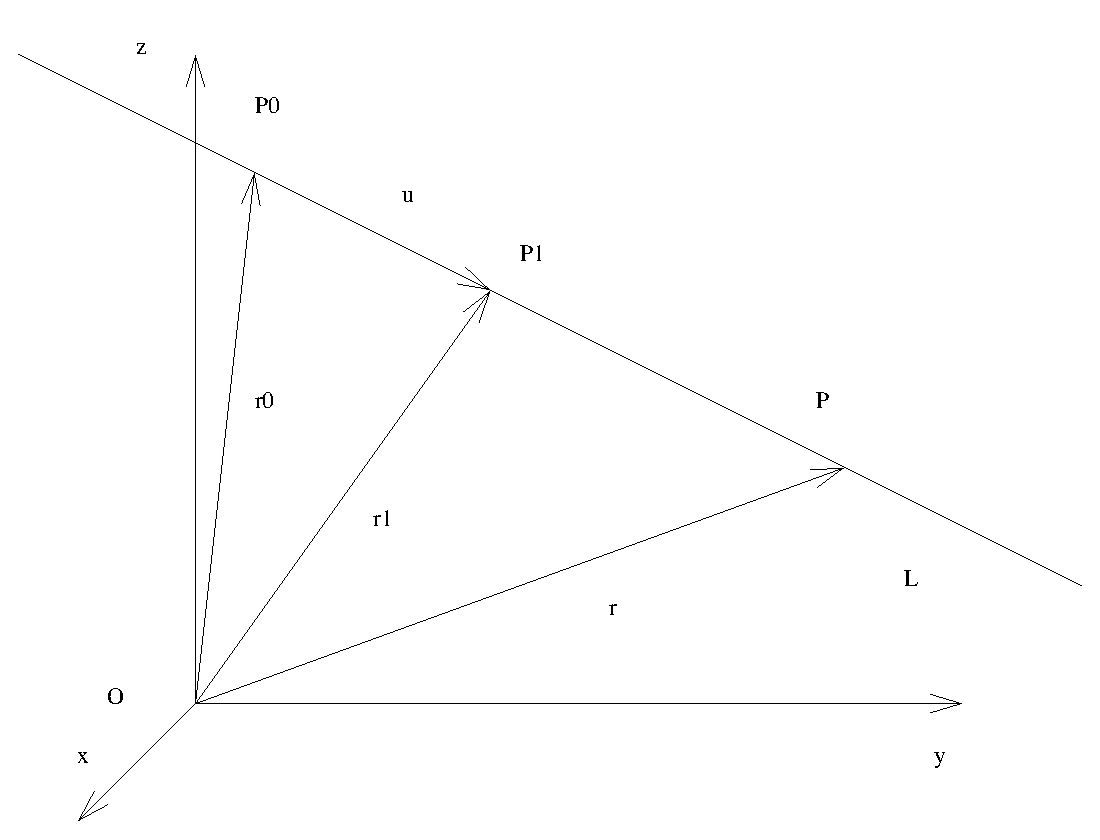
\includegraphics[height=1.5in]{../../modules/vectors/pictures/ok-line_point_point_scalar.eps}
    \end{figure}}
\end{columns}

\uncover<5->{\textcolor[rgb]{0.98,0.00,0.00}{Parametric scalar equations}:
%
$$\left\{ \begin{array}{ll}
           x & = x_0 + t(x_1-x_0) \\
	   y & = y_0 + t(y_1-y_0) \\
           z & = z_0 + t(z_1-z_0)
          \end{array}
\right. \leftrightarrow \left\{ \begin{array}{ll}
           x & = (1-t)x_0 + tx_1 \\
	   y & = (1-t)y_0 + ty_1 \\
           z & = (1-t)z_0 + tz_1
          \end{array}
\right. , \quad t \text{ real number.}$$}
\end{frame}


\begin{frame}
 \frametitle{Example}

Line $L$ through $P_0(1,2,3)$ and $P_1(5,2,1)$.

\begin{itemize}
 \item<2-> Direction of $L$: $\textbf{u} = \textbf{r}_1-\textbf{r}_0 = \langle 4, 0, -2\rangle$.
\item<3-> Parametric vectorial equation:
%
$$\textbf{r} = \langle 1,2,3\rangle + t \langle 4, 0 -2\rangle \leftrightarrow \textbf{r} = \langle 1+4t, 2, 3-2t\rangle\; .$$
%
\item<4-> Parametric scalar equations:
$$\left\{ \begin{array}{ll}
           x & = 1+4t \\
	   y & = 2 \\
           z & = 3-2t
          \end{array}
\right. , \quad t \text{ real number.}$$
%
\item<5-> Symmetric equations:
%
$$\frac{x-1}{4} = \frac{z-3}{-2} \quad \text{ and } \quad y=2\; .$$
\end{itemize}

\end{frame}